
%\documentclass{IEEEtran}%{sig-alternate-10pt} %{usetex-v1} %[11pt,twocolumn]{article}
\documentclass[10pt]{article}
\usepackage{graphicx}
\pagenumbering{gobble}

\usepackage[margin=0.5in]{geometry}

\begin{document}
\section{Personalized News Feeds}
\subsection{Recommendation's news feed}
I created a new feed using the following terms in the Google news: 
\begin{itemize}
\item{Recommendation Systems}
\item{Recommender Systems}
\item{Online Recommendation}
\end{itemize}
besides the edition is set to US, and the category to Technology. Since I was interested to news in all languages I did not choose any specific language. 

\textbf{Feedback}: Figure \ref{recfeed}, contains the an snapshot of the first eight feeds  of the founded news at the date of 5 October 2013. In the list of news, the 1st, 4 5 6 7th are relevant to what it is meant of recommendation in this course. The 2nd and 3rd news appear since the term "recommendation systems" appears in the body of the news, but they are not directly about recommendation systems. I think, one of the reasons for this mis-ranking is that those feeds are new and they get upper places in the list on feeds.

\begin{figure}[h]
\begin{center}
    \centering 
    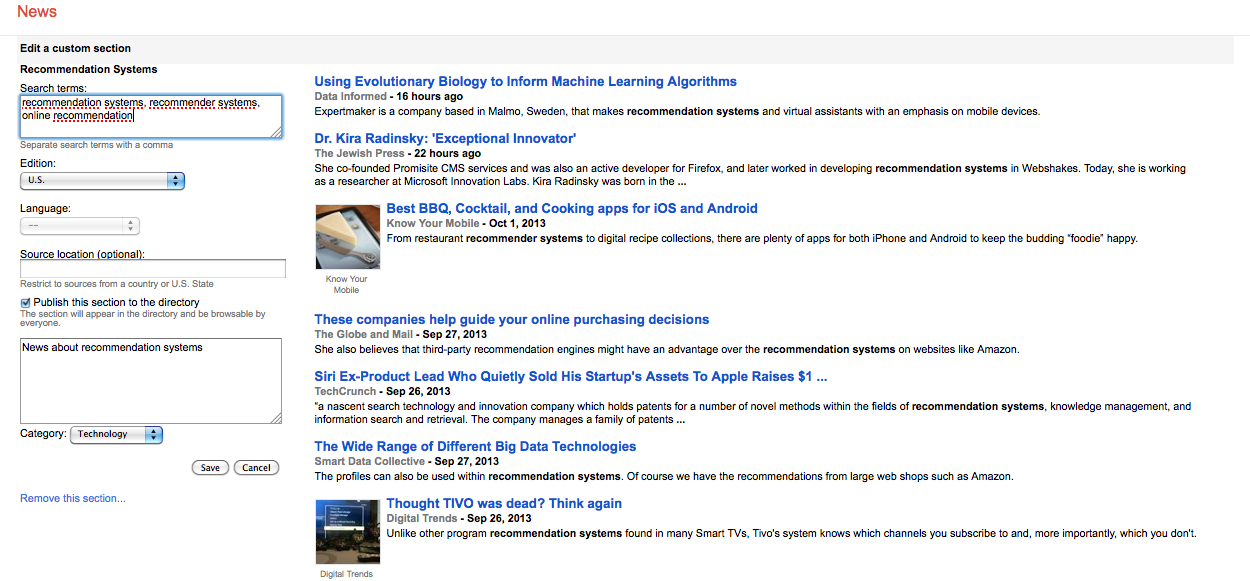
\includegraphics[scale=.52]{pic2.png}
    \caption{An snapshot of the recommendation news feed}
    \label{recfeed} 
\end{center}
\end{figure}




\subsection{Tennis Rank's news feed}
Since I was interested to tennis game, I made a news feed about tennis players ranks. First, I used the following terms in the built of the feed.

\begin{itemize}
\item{Grand Slam}
\item{WTA Tennis}
\item{Rennis Ranking}
\item{Best Tennis Players}
\end{itemize}
with these terms I get the following news at the date of 5 October 2013. 

\begin{figure}[h]
\begin{center}
    \centering 
    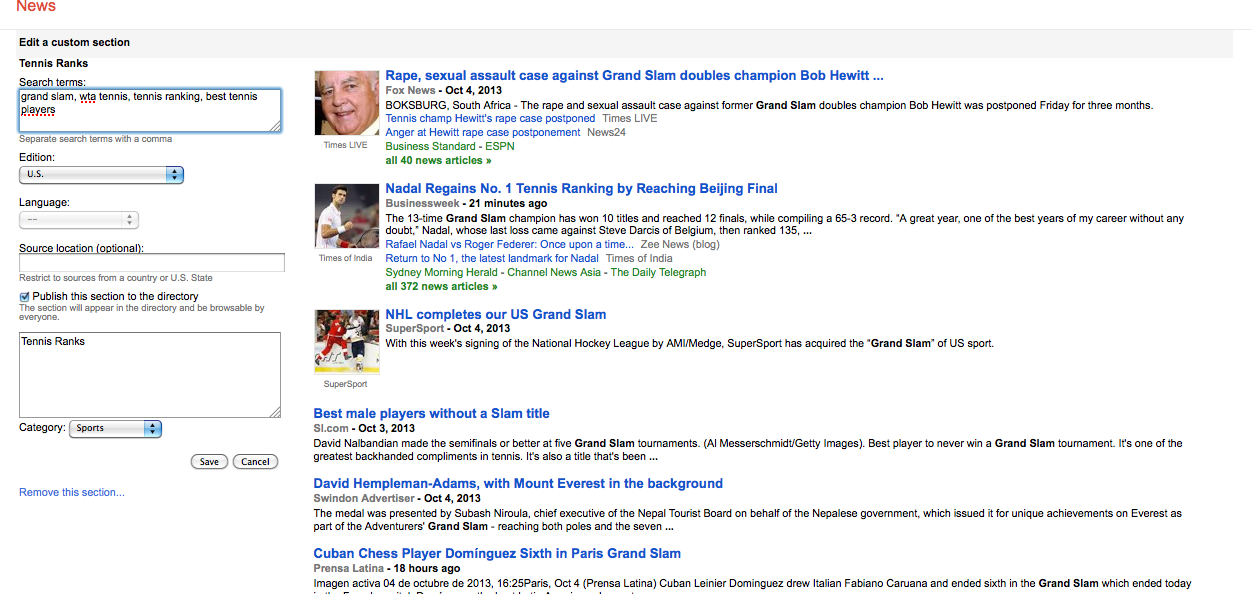
\includegraphics[scale=.52]{pic3.png}
    \caption{An snapshot of the initial tennis news feed}
    \label{tennisfeed} 
\end{center}
\end{figure}

\textbf{Feedback}: As the Figure \ref{tennisfeed} shows most of the news are unrelated to tennis game, and it is due to the first term \emph{grand slam}. Not only tennis but some other popular games have grand slam competitions, so this term is not a proper term for this type of feed. To fix it, I modified the search terms and removed the "grand slam" and get a better result, see Figure \ref{tennisfeedBetter}.

\begin{figure}[h]
\begin{center}
    \centering 
    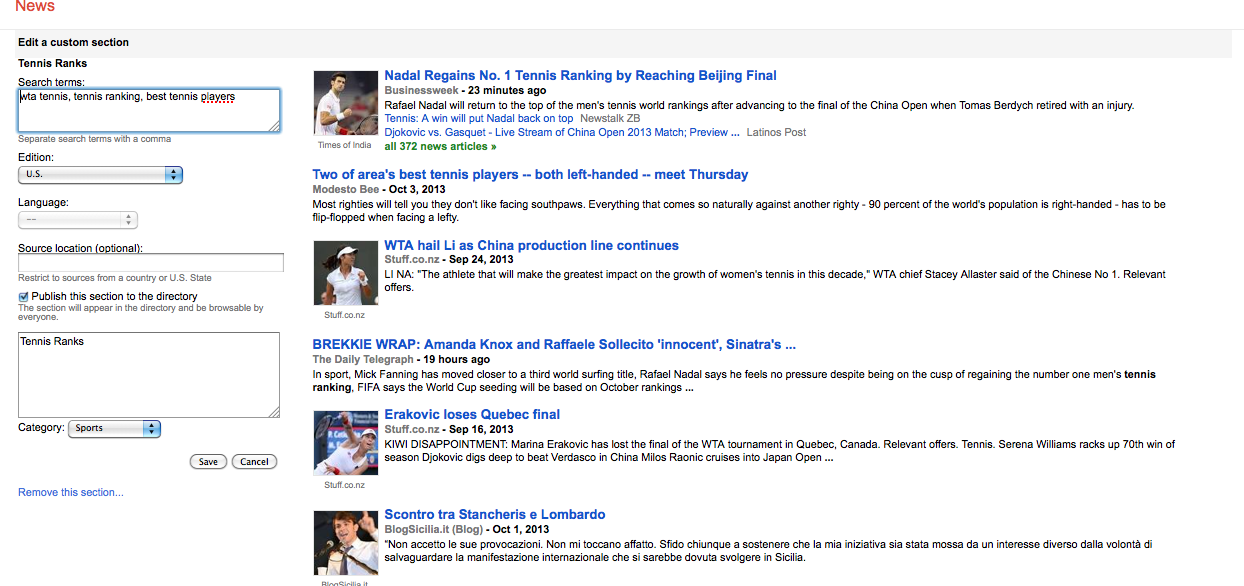
\includegraphics[scale=.52]{pic33.png}
    \caption{An snapshot of the modified tennis news feed}
    \label{tennisfeedBetter} 
\end{center}
\end{figure}




\subsection{Flower business's news feed}
I was interested to see how Google's news service can find feeds about the "flower business". I used the following terms to make such a feed:

\begin{itemize}
\item{Flower import/export}
\item{Flower business}
\item{Flower trade}
\item{Flower market}
\item{Flower Stock}
\end{itemize}

\begin{figure}[h]
\begin{center}
    \centering 
    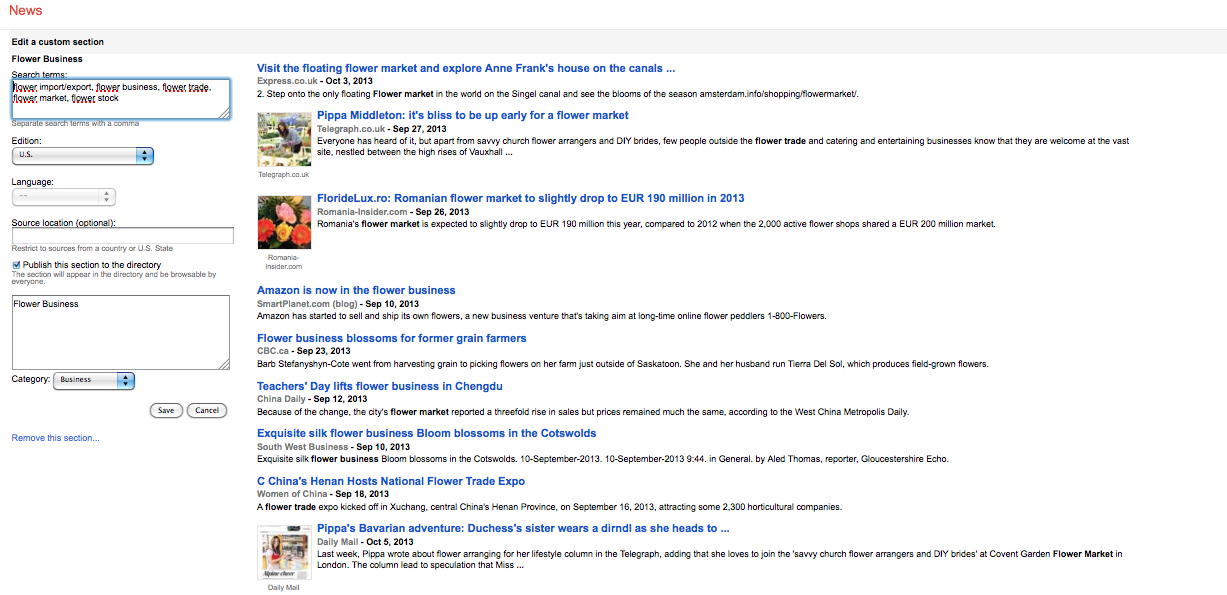
\includegraphics[scale=.52]{pic4.png}
    \caption{An snapshot of the flower business news feed}
    \label{flowerBusiness} 
\end{center}
\end{figure}

Figure \ref{flowerBusiness} contains an snapshot of the feed, taken at 5 October 2013.

\textbf{Feedback}: As it is seen from the feeds, Figure \ref{flowerBusiness}, except for the 1st feed which not exactly about the flower business, the rest more or less are. It seems that the term "flower market" is not a proper term, it mainly refers to local flower market in the cities. Besides, I noticed that the "flower import/export" has not been used in any of the feeds, so the way that this term is expressed should be modified as well. I applied these modifications and I got better results, see Figure \ref{flowerBusinessBetter}.

\begin{figure}[h]
\begin{center}
    \centering 
    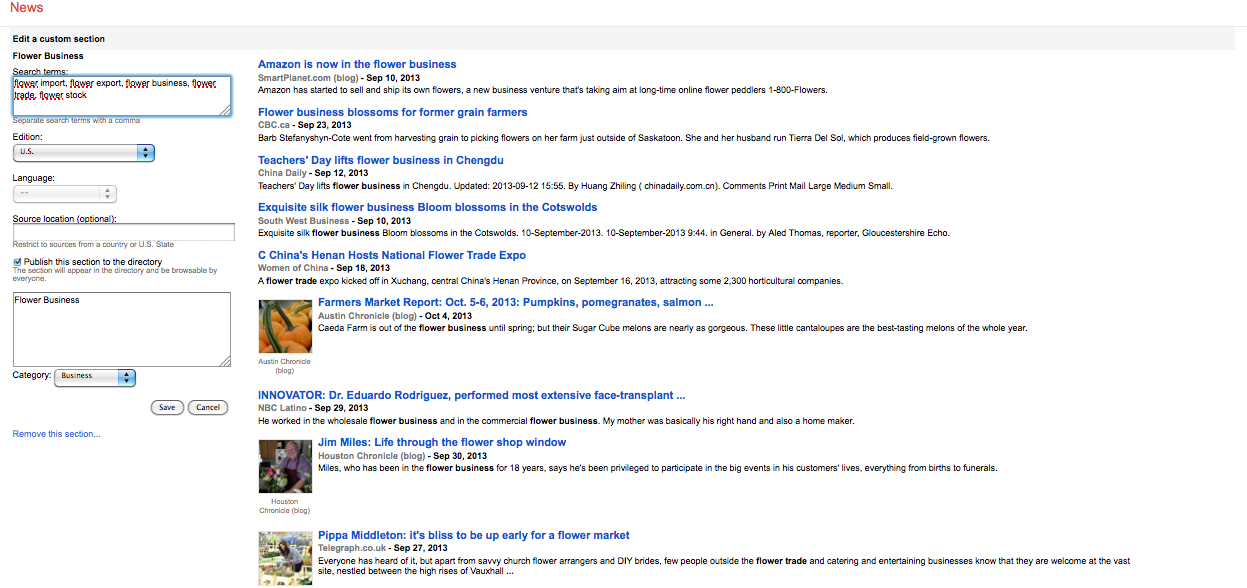
\includegraphics[scale=.52]{pic5.png}
    \caption{An snapshot of the improved flower business news feed}
    \label{flowerBusinessBetter} 
\end{center}
\end{figure}


\end{document}